\documentclass[10pt]{scrartcl}

\usepackage{graphicx}
\usepackage{subcaption} 
\usepackage{float}
\usepackage{nameref}
\usepackage{hyperref}
\usepackage{color,soul}

\title{Scientific Experimentation and Evaluation\\
		\small{Assignment 7}}
\author{Chaitanya Hebbal\\
		Jos\'e Carlos Mayoral Ba\~nos}

\begin{document}
	\maketitle
\section*{Task Description}

Using a modified LEGO robot from the experiment \textit{"Manual motion observation"} a new set of poses will be acquired via AICISS lab optical localization system, then the data will be analyzed to observe the variation on the poses and look at the error distributions in order to observe the variation on the measures and look at the error distributions.

The layout of this experiment consists on:
\begin{enumerate}
	\item Five different curves movements are going to be measured: Straight line and 4 arcs (2 left and 2 right).
	\item The Device Under Test is a modified LEGO robot from the experiment \textit{"Manual motion observation"}.
\end{enumerate}

\section*{AICISS Lab Optical Localization System}

A optical-based localization system will be used in this experiment. From \cite{OptSystem} the optical systems have several advantage to take into account:

\begin{itemize}
\item Less susceptible to noise from the environment. 
\item Optical tracking does not suffer from drift problems.
\item Optical tracking allows for many objects to be tracked simultaneously.
\item Interaction devices can be lightweight and wireless. 
\end{itemize}

%\begin{figure}[h!]
%\centering
%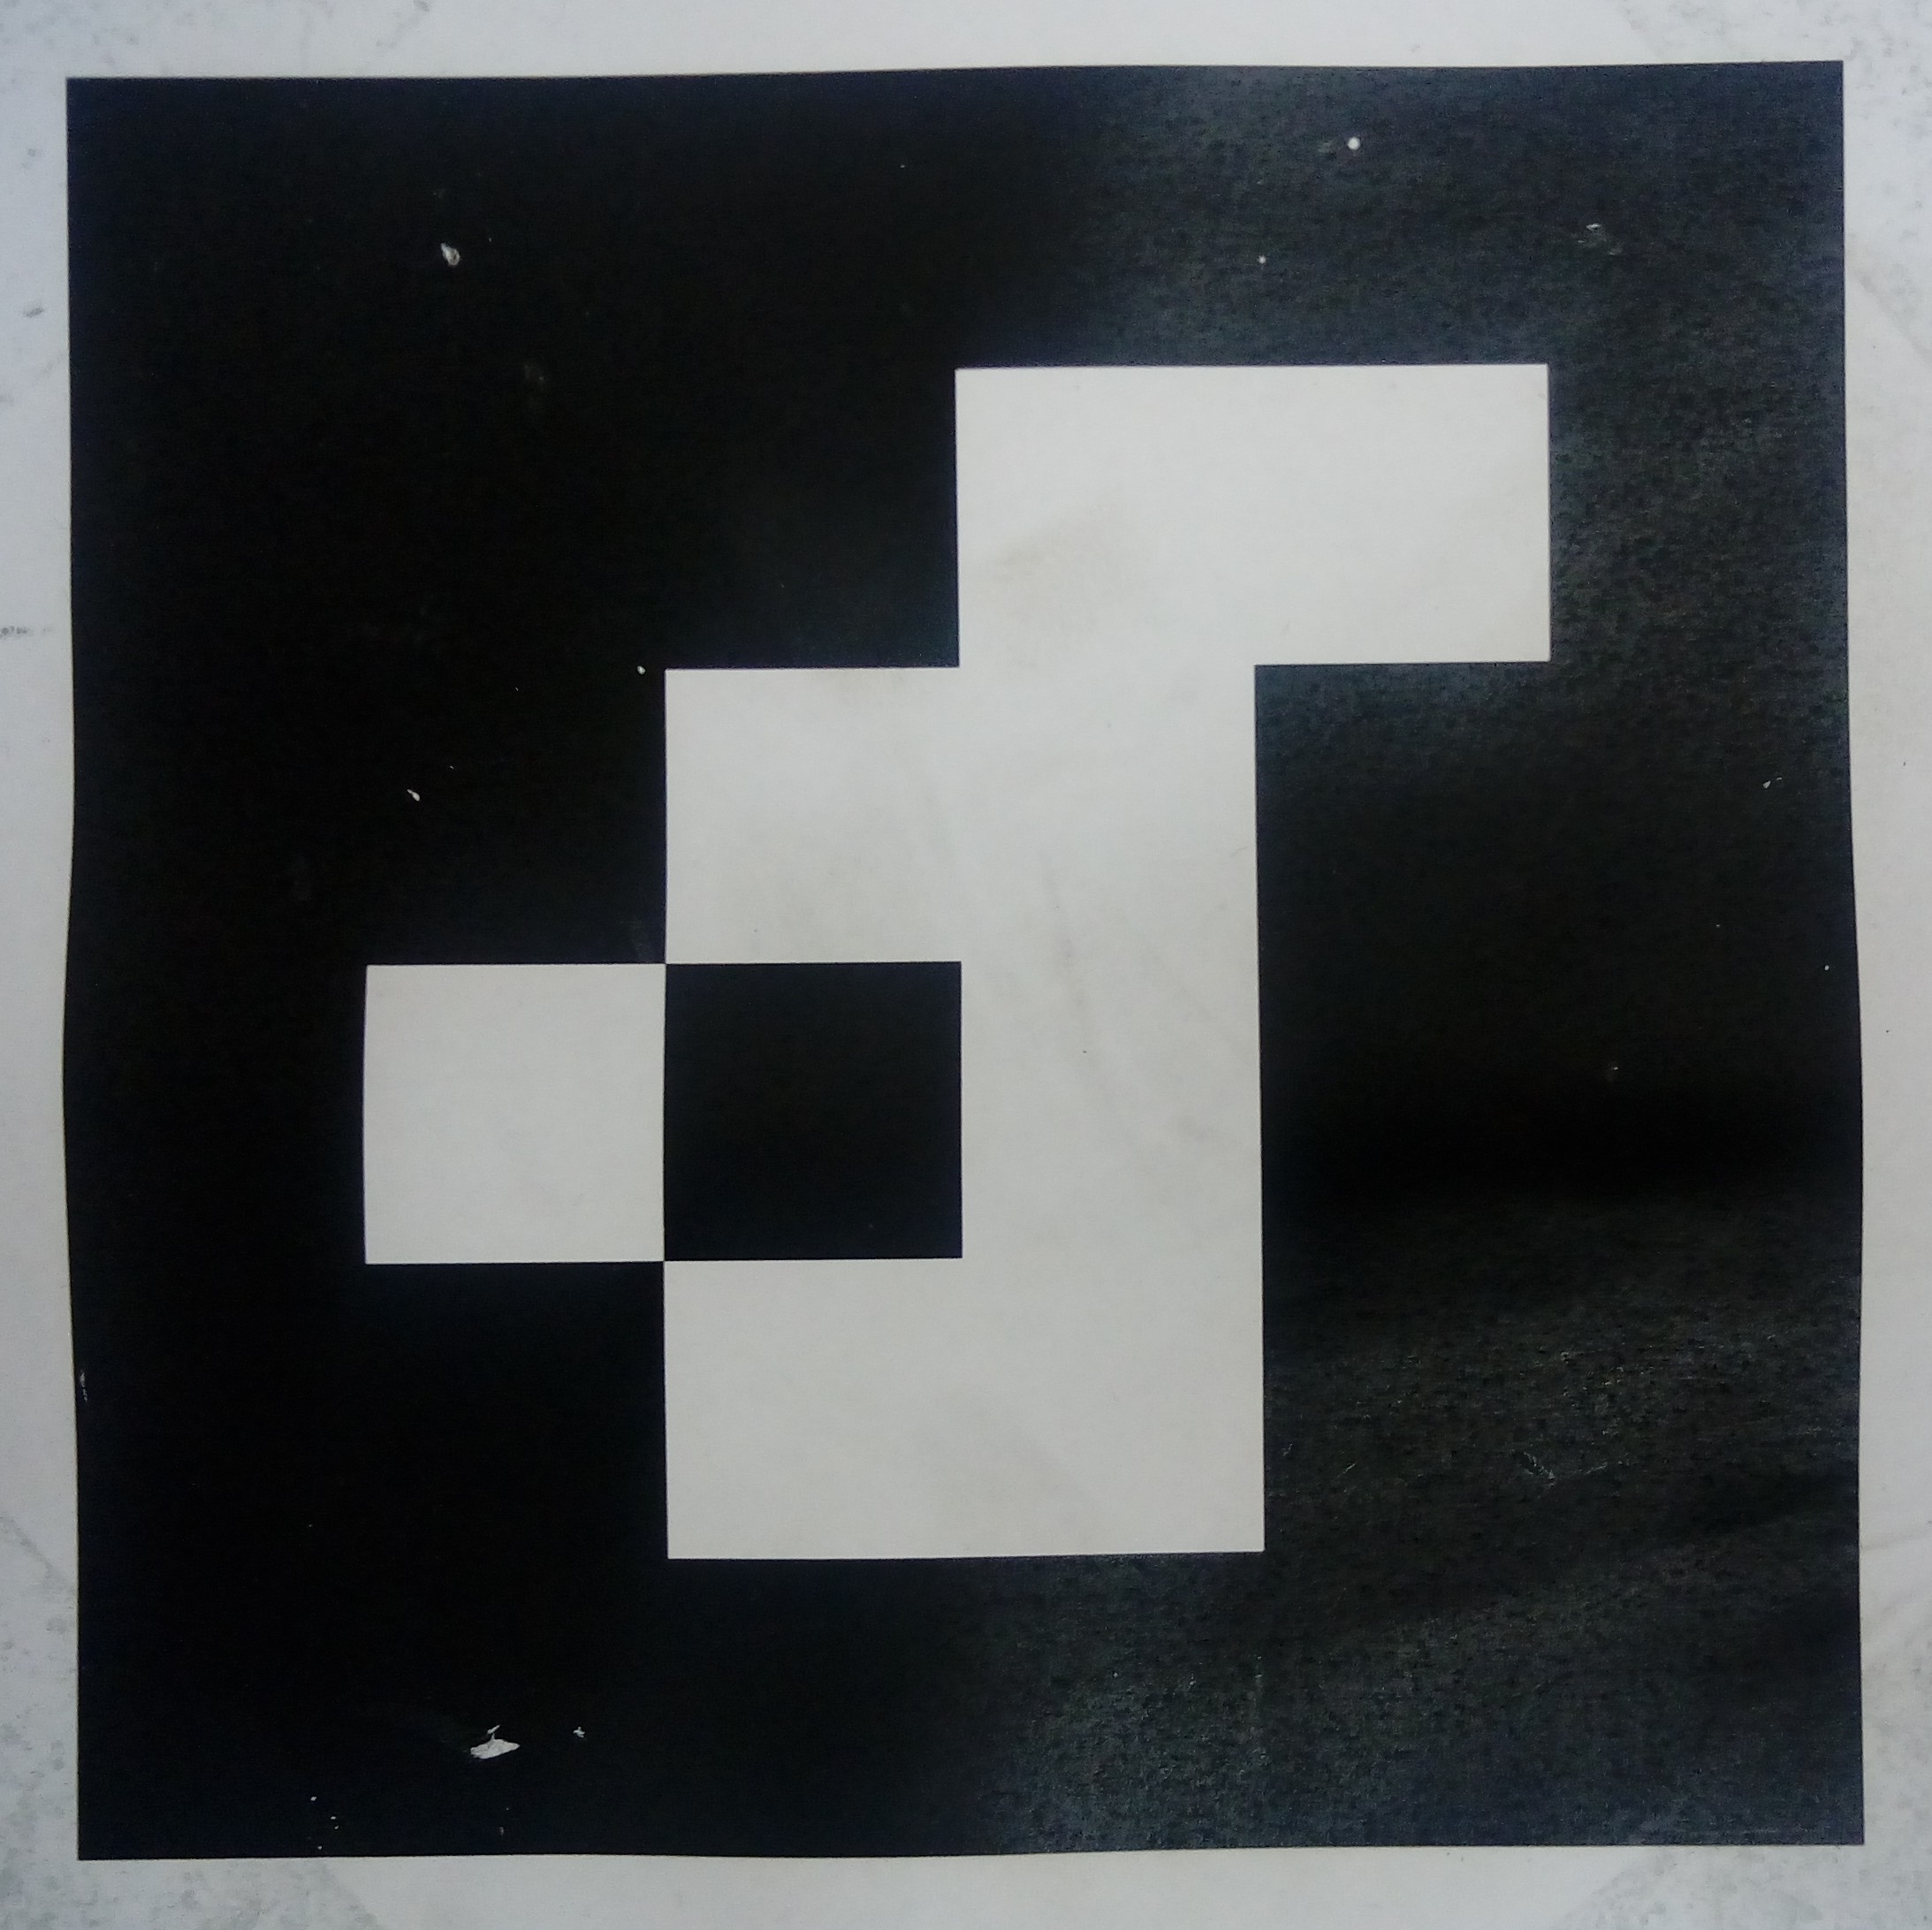
\includegraphics[angle=-90,scale=0.5]{images/marker}
%\caption{AICISS Cameras}
%\label{fig:cameras}
%\end{figure}


Therefore, at AICISS Lab there is already an "Optical Localization System" which uses several cameras in order to track pre-defined markers, such as the one shown at figure \ref{fig:marker}. By adding multiple cameras to the tracker system the precision of each pose increases and the system becomes more accurate. The AICISS system uses 3 cameras and a single workstation manages it. The workspace area sizes 7.3 meter width and 3.5 height.

\begin{figure}[h!]
\centering
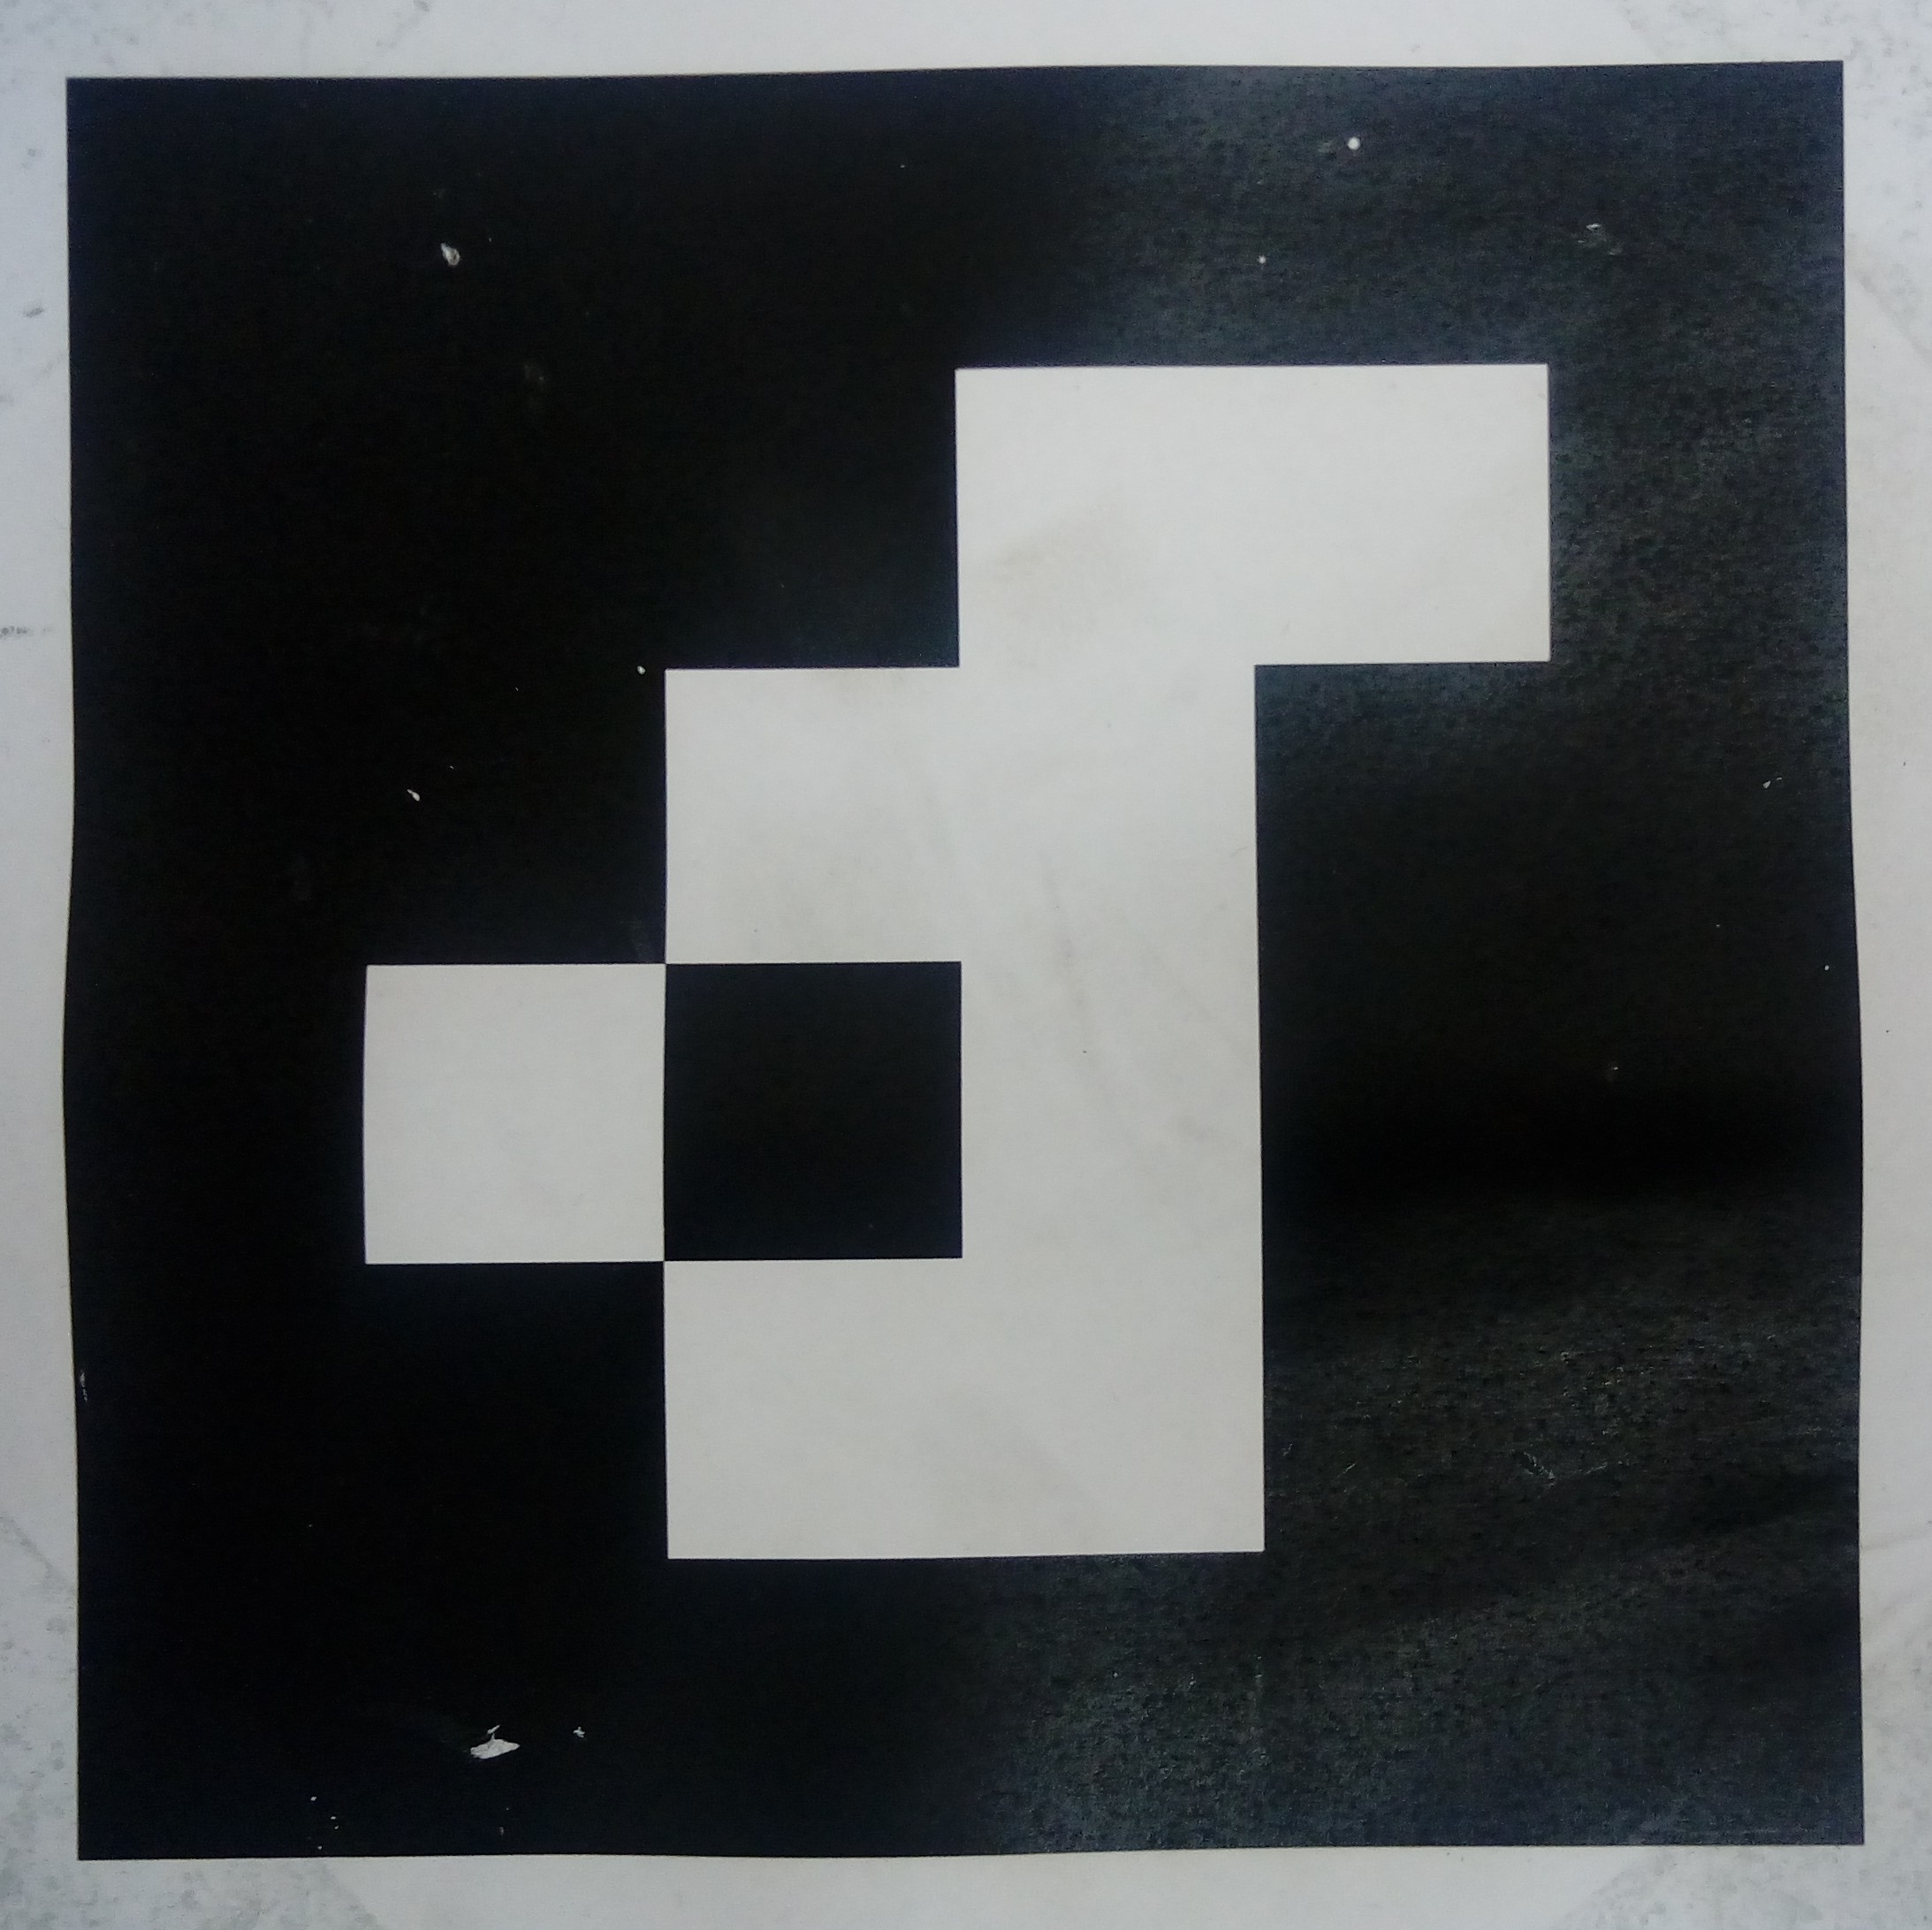
\includegraphics[angle=-90,scale=0.05]{images/marker}
\caption{AICISS Marker}
\label{fig:marker}
\end{figure}

Speaking about software, it has some components that need to be run in the workstation for the tracking system. It is important to mention that the output data of the system is a pose array with time stamps therefore the system provides additional data in comparison with manual measurements process.

\begin{itemize}
	\item 'camera\_server': Run the cameras.
	\item 'robot\_tracker': Run the tracker service.
	\item 'apt-robot $>>$ your\_file.log': In case a log file which stores all the data is needed.
	\item '': Open a visualization interface.% (figure \ref{fig:visualizator}).
\end{itemize}

%\begin{figure}[h!]
%\centering
%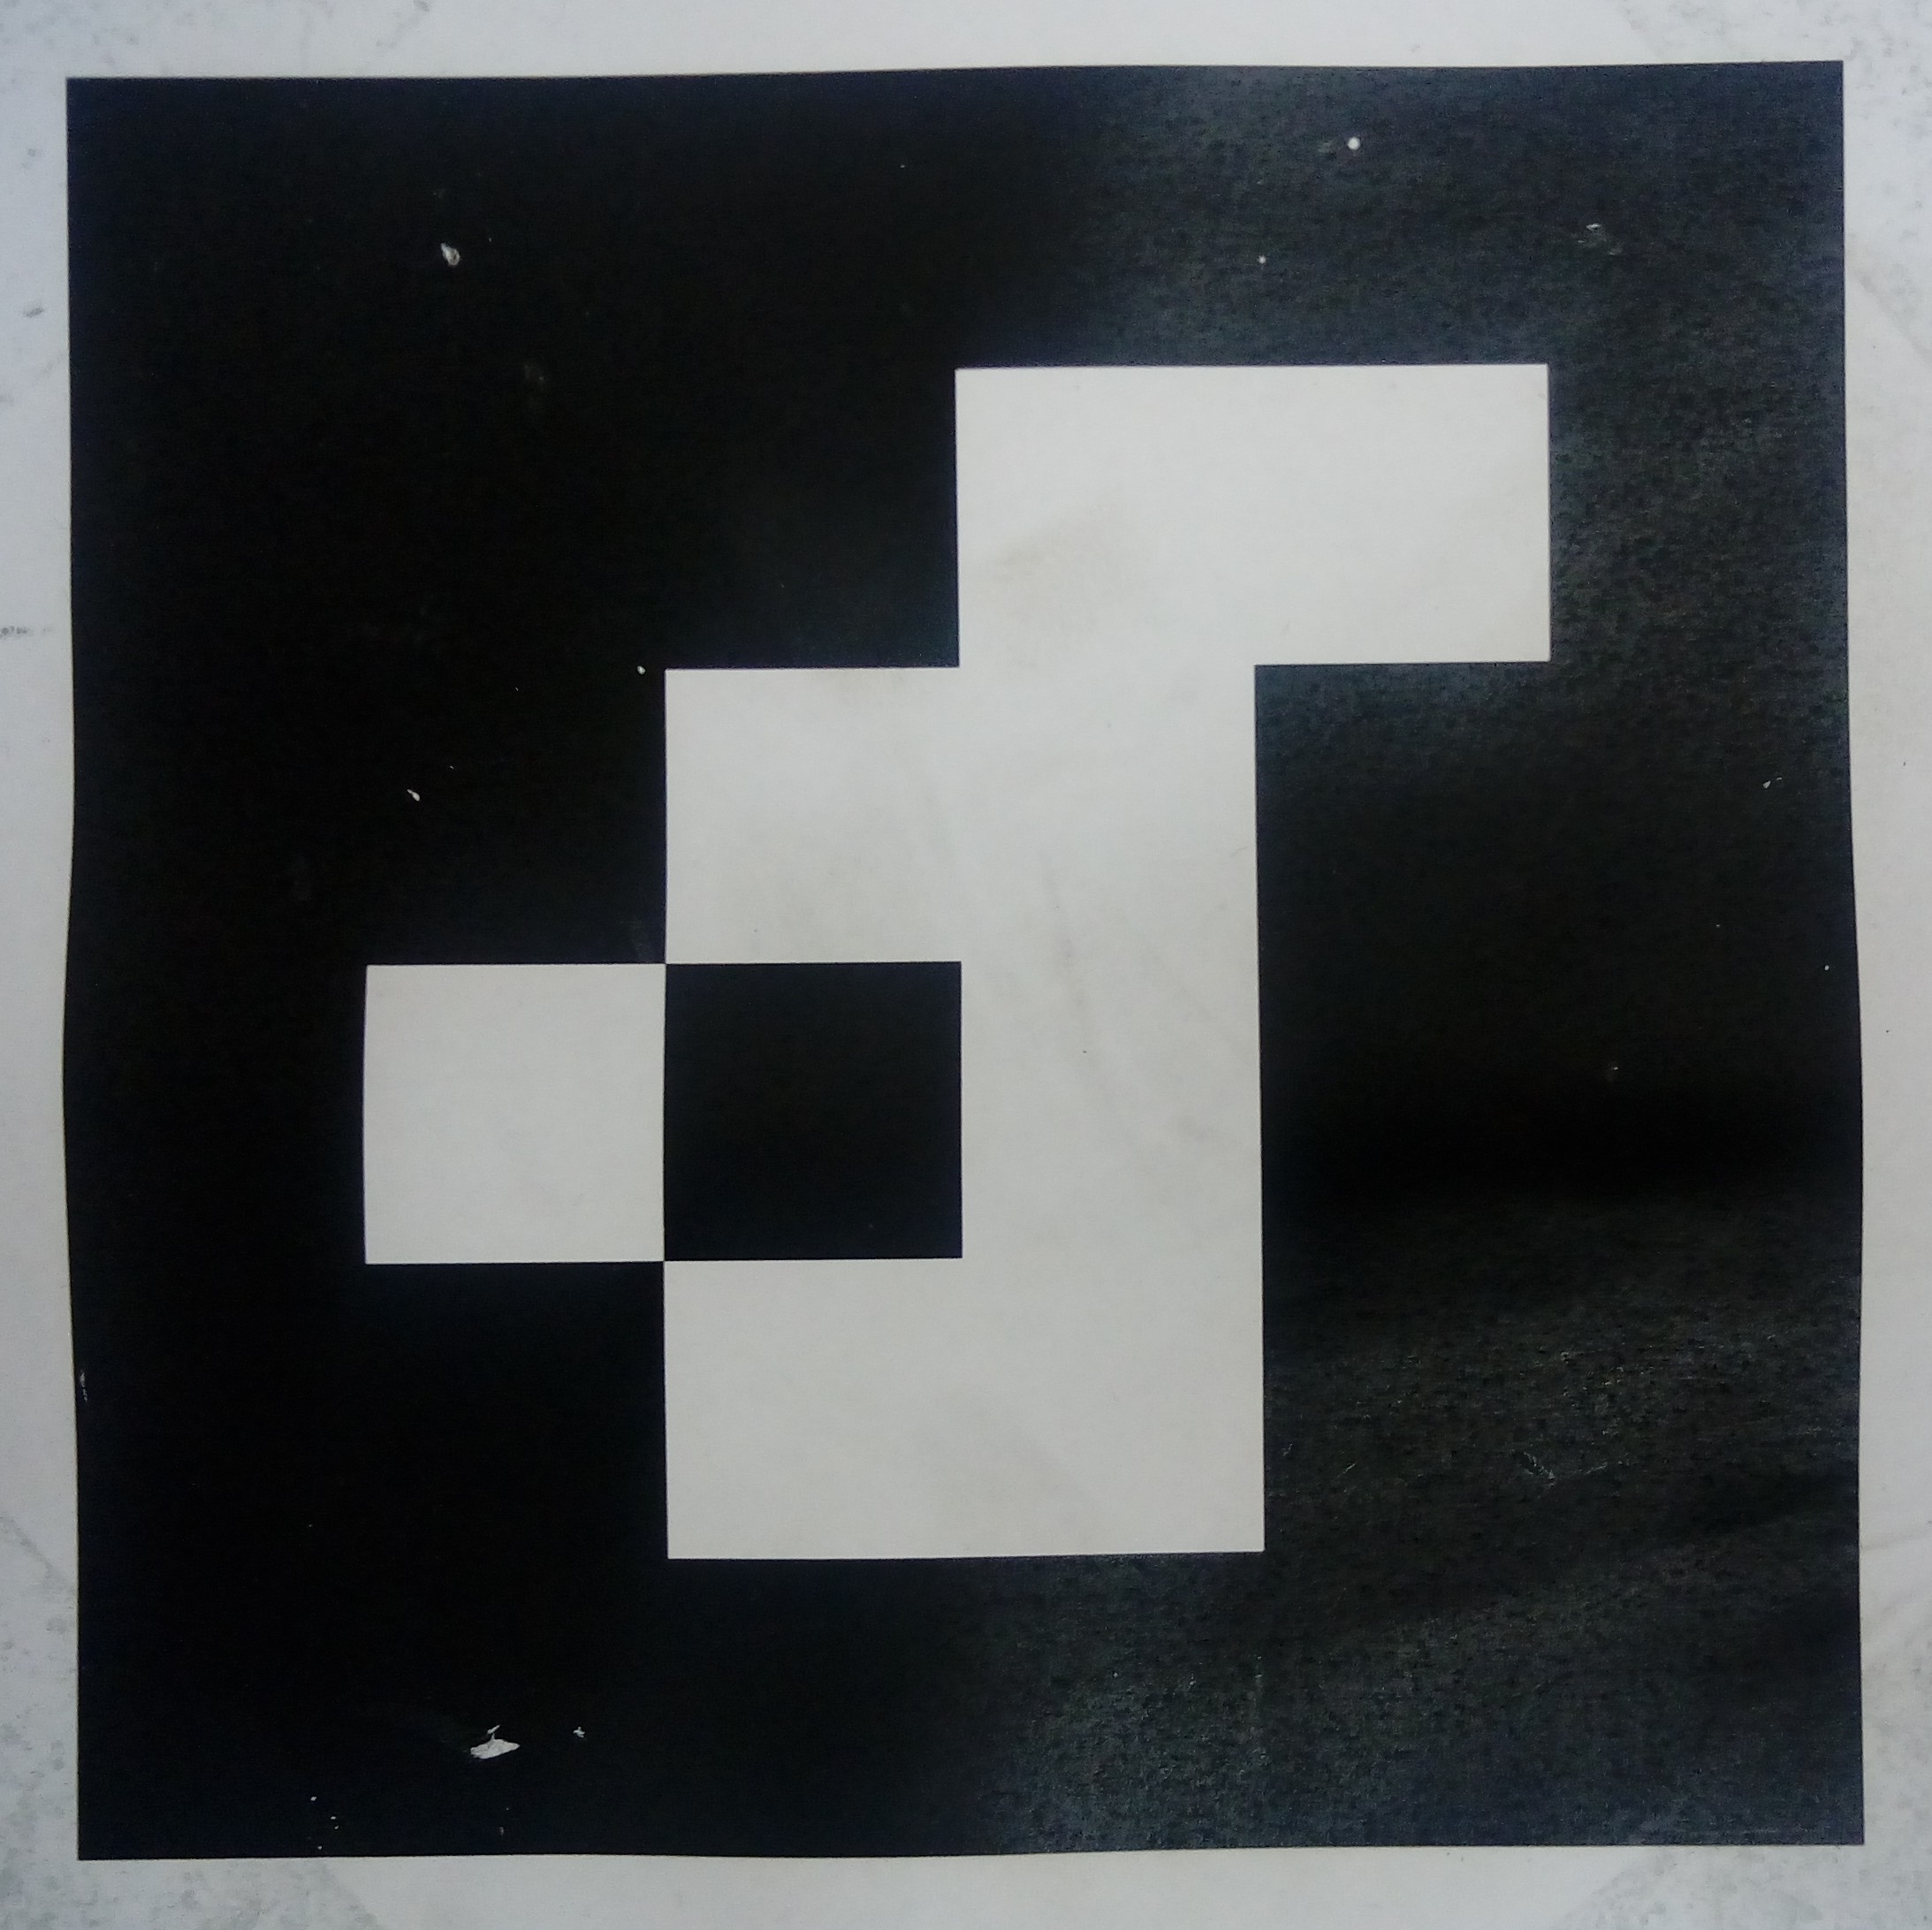
\includegraphics[angle=-90,scale=0.5]{images/marker}
%\caption{Optical System Visualizator}
%\label{fig:visualizator}
%\end{figure}

\section*{Experiment setup}

\subsection*{Device Under Test}

A tracker have been added to the top of the robot in order to make able the system to track it, the robot configuration is shown at figure \ref{fig:1}.

\begin{figure}[ht!]
\centering
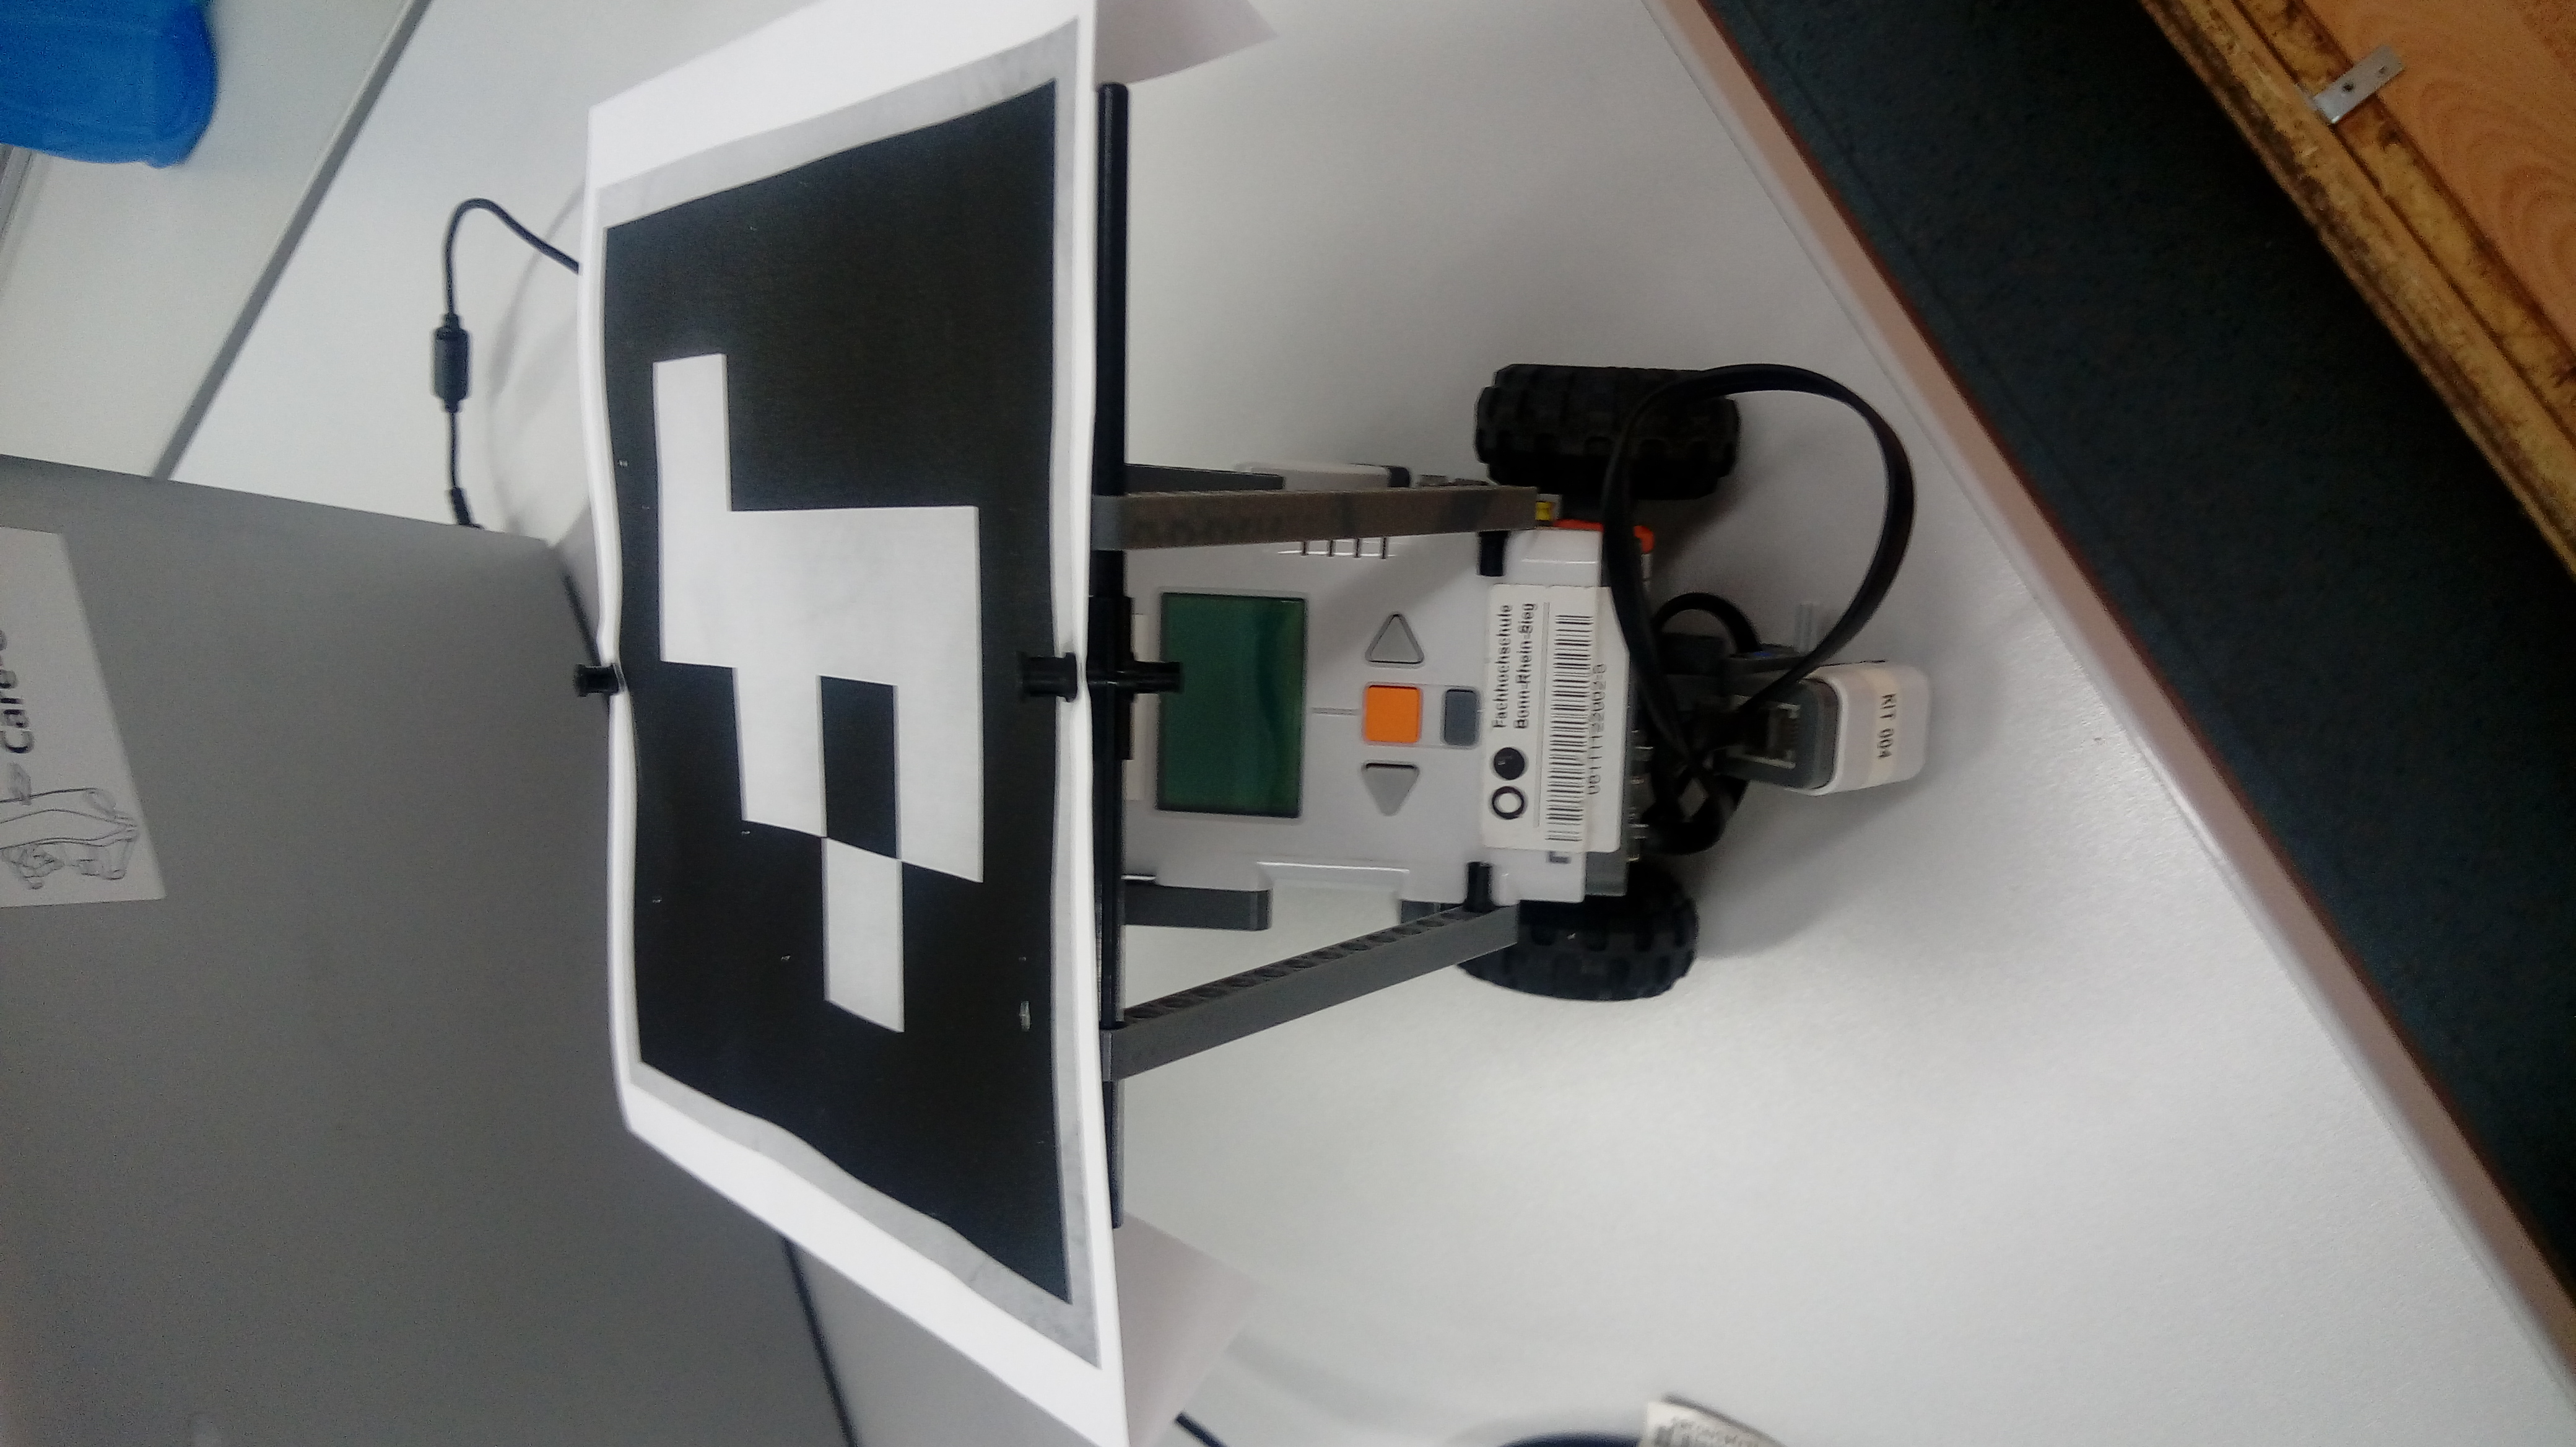
\includegraphics[angle=-90,scale=0.05]{images/robotWithMarker}
\caption{LEGO Nxt Robot}
\label{fig:1}
\end{figure}

\subsection*{Measuring Method}

The measuring method for each curve consists on:
\begin{enumerate}
	\item The component camera\_server and robot\_tracker must be running.
	\item Two light sensors are used to mark the points in order to get the pose of the robot.
	\item One example of the marker is shown at image \ref{fig:initMatcher}.
	\item After localizing the robot, the apt-robot component runs before the robot starts movement.
	\item Click robot left button to start robot movement.
	\item After the robot stops, the apt-robot component is stopped.
	\item The robot location changes by hand to the initial pose.
	\item Repeat 40 times steps from 4 to 7.
\end{enumerate}

\begin{figure}[ht!]
\centering
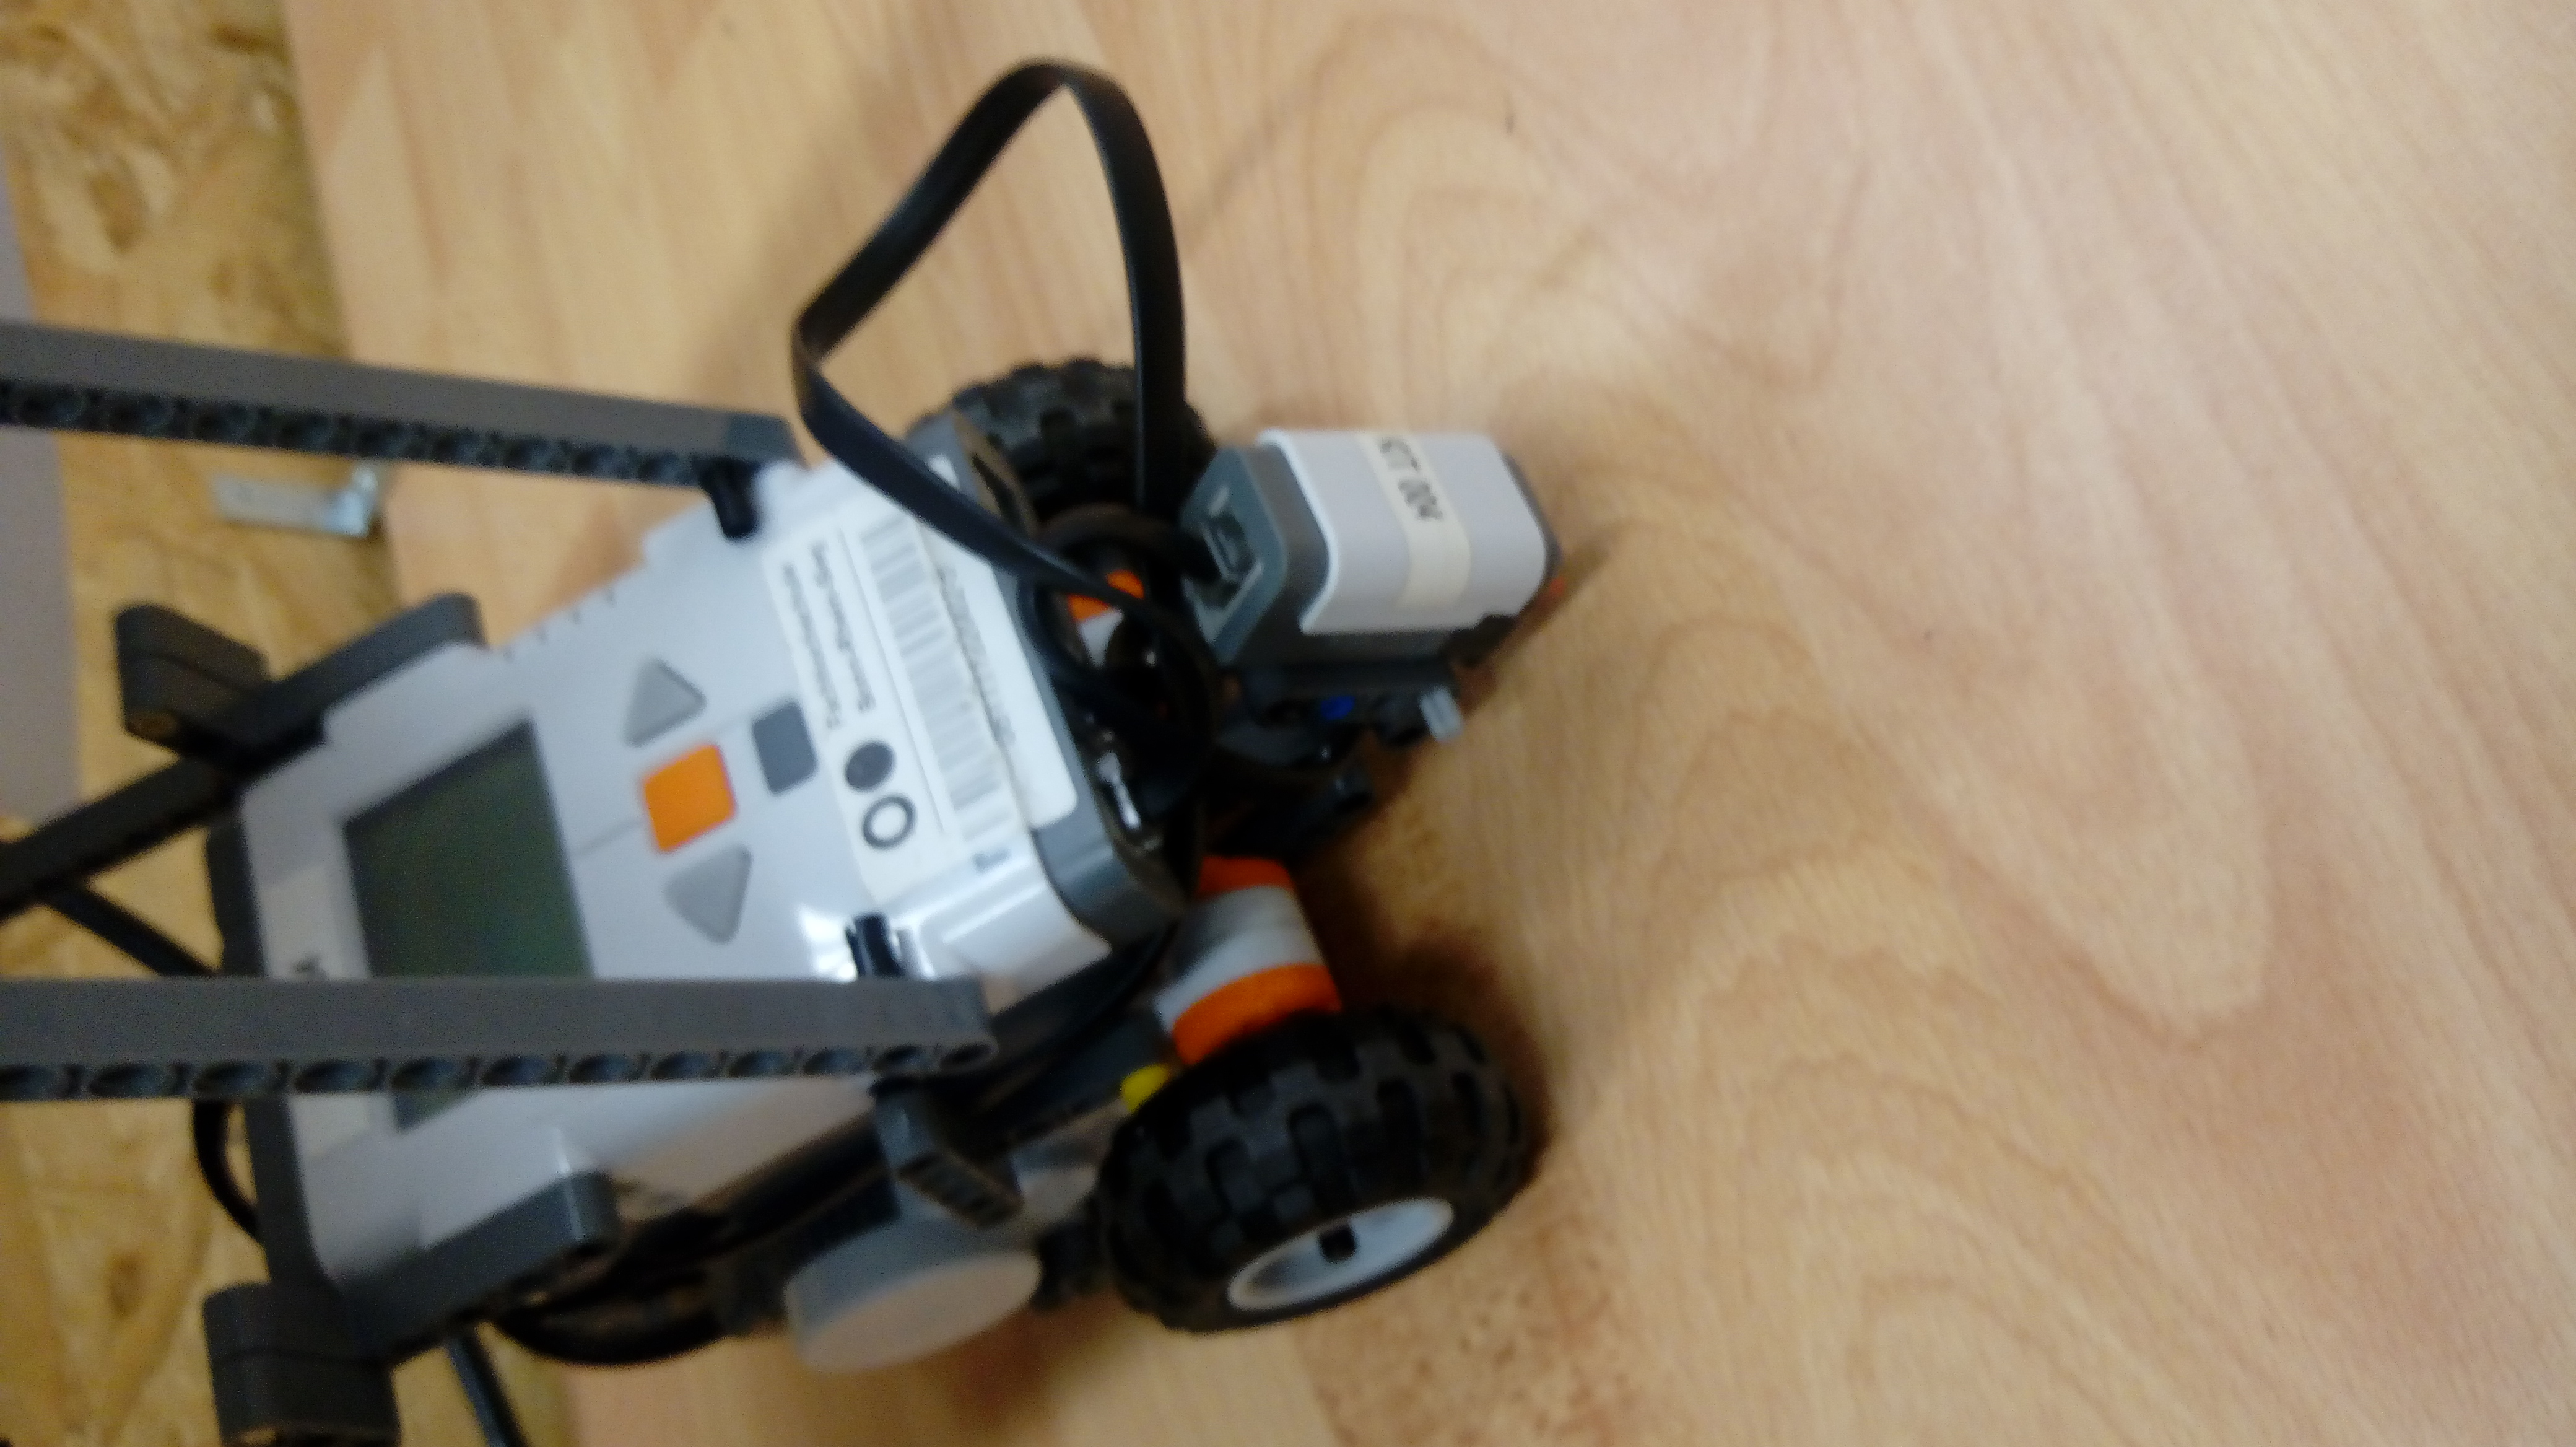
\includegraphics[angle=-90,trim={1200 700 1000 300},clip,scale=0.10]{images/initChecker}
\caption{One mark per laser is marked on the floor with a pencil to start at the same pose}
\label{fig:initMatcher}
\end{figure}


\subsection*{What difficulties are expected?}

\begin{itemize}
	\item Other tracker in the arena must be hidden.
	\item The initial pose markers don't guarantee the same initial pose.
	\item Tracker can loses the robot for instances then the data is not noise-free.
\end{itemize}


\subsection*{Data Processing}

The raw measurements are shown at figure \ref{fig:realScaleraw}. This figure doesn't show any kind of data processing so it makes able to see some noisy measurements that don't relies to any of the five curves. Also the figure shows an unexpected problem with a measurement method which is that the curve were acquired in two different days then the initial marker were lost for the second day. In the figure, straight and slightleft curve were taken in the first day, the rest on the second one.

%\begin{figure}[ht!]
%\centering
%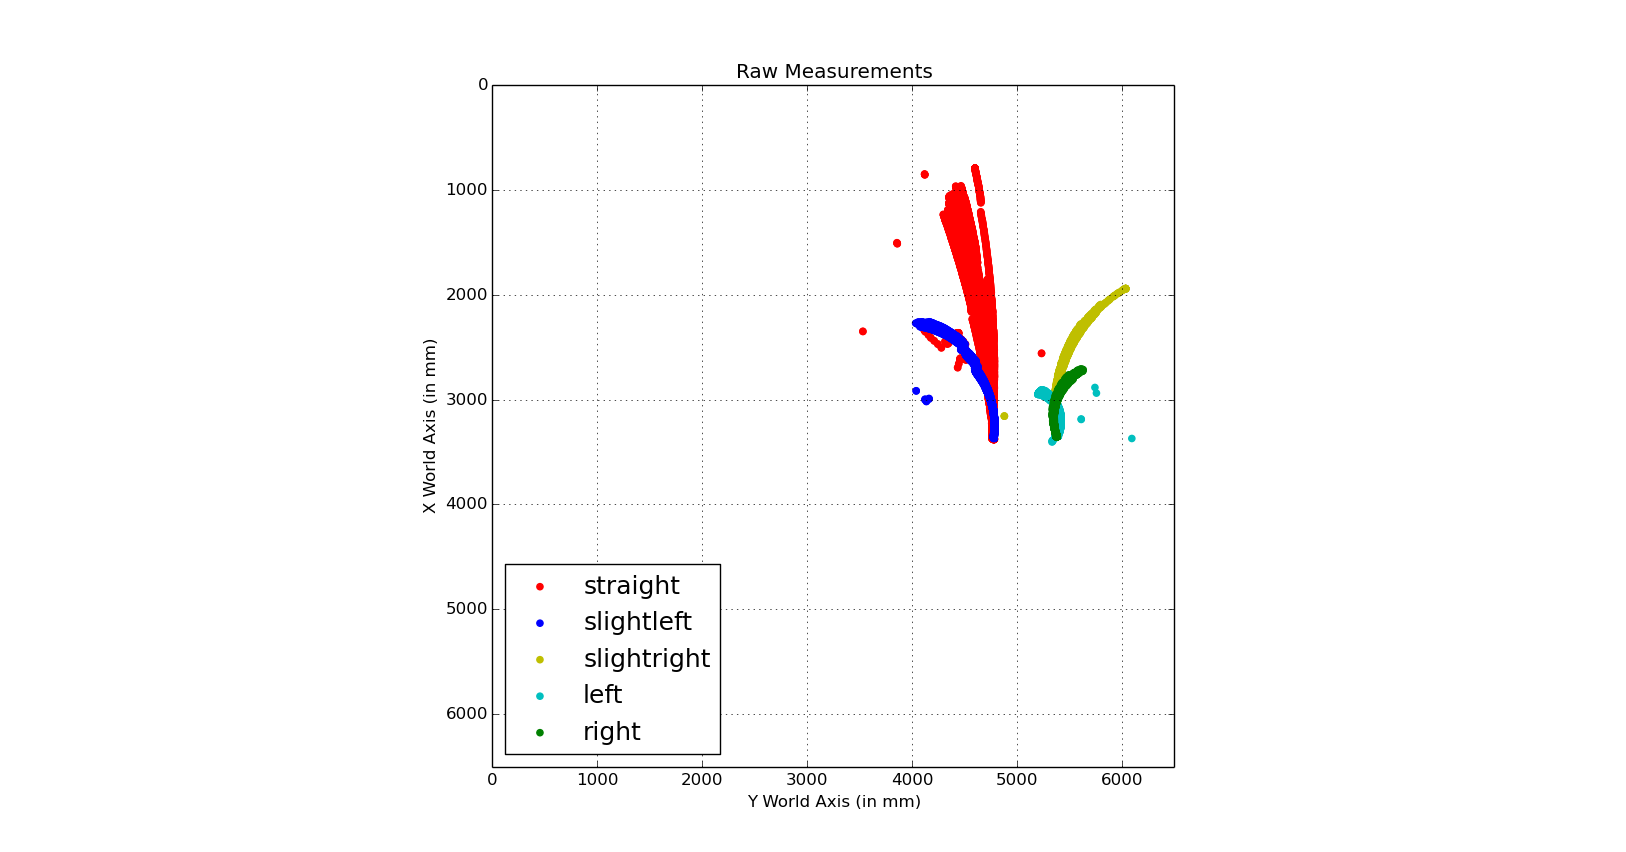
\includegraphics[trim={200 0 0 0},clip,scale=0.50]{images/rawMeasurements}
%\caption{Raw Acquired Data}
%\label{fig:rawMeasurements}
%\end{figure}

%However the figure \ref{fig:rawMeasurements} doesn't show the real size of the environment. The correct scale is shown at \ref{fig:realScale}.

\begin{figure}[ht!]
\centering
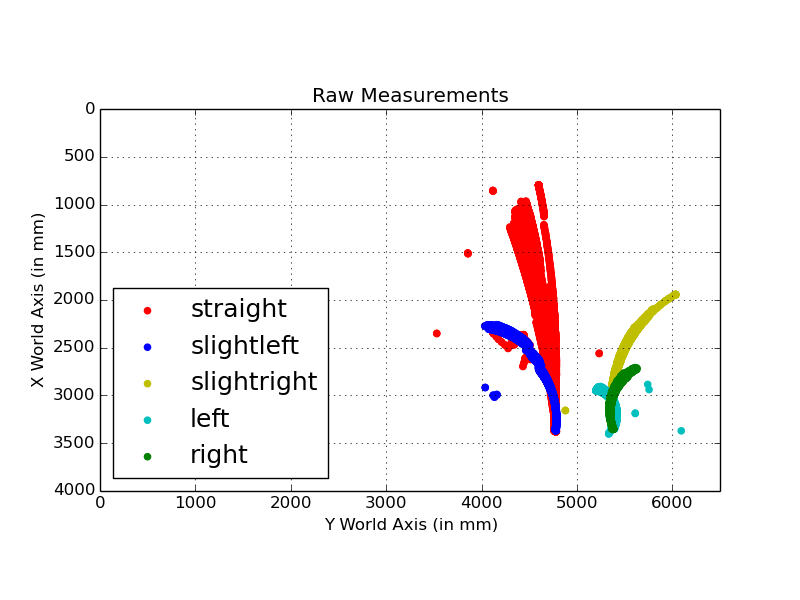
\includegraphics[scale=0.50]{images/realScaleraw}
\caption{Raw Acquired Data}
\label{fig:realScale}
\end{figure}

All the data has different starting point due to the fact that even using a start pose markers it still not be so accurate and the number of samples for each measurement are not the same. So for every curve there are 40 possible initial poses then:

\[	
	\bar{p_0} = \frac{1}{n} \sum_{i=1}^{n} p_{i_0}
\]
where $n = 1,2,\cdots 40$ and $i_0$ is the first pose of each measurement.

Then this calculated initial pose was substracted to all the poses from the files.
\[	
	\hat{p_m} = p_m - \bar{p_0}
\]
Additionally the sizes of the measurements files were trim to the minimum length of all of the measurements. The result project all measurements to the origin of a frame \ref{fig:preprocess}.

\begin{figure}[ht!]
\centering
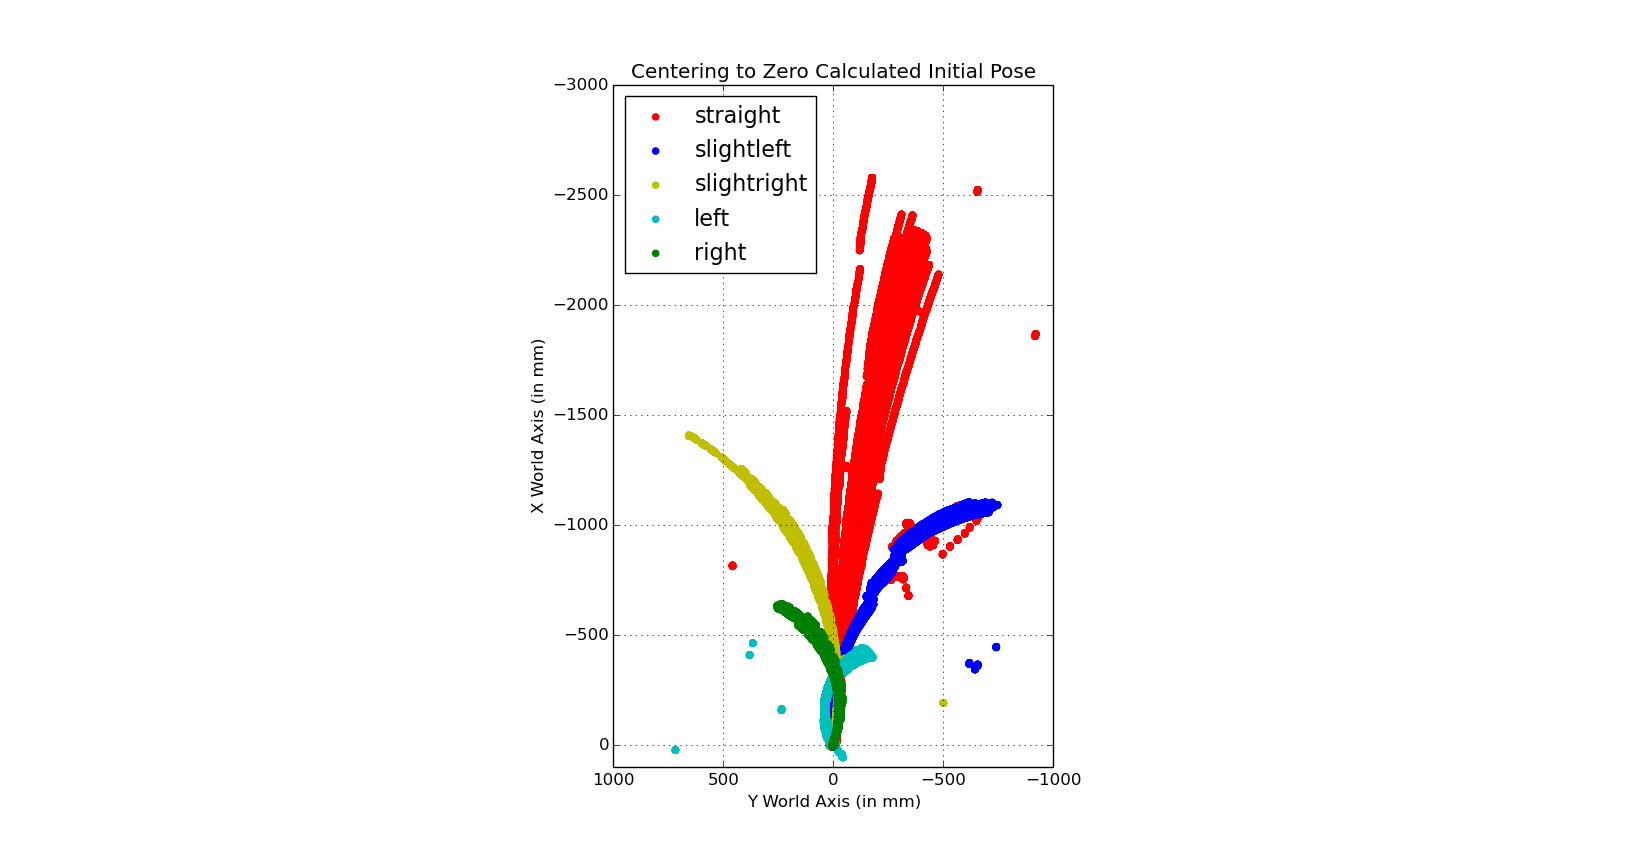
\includegraphics[trim={220 0 0 0},clip,scale=0.5]{images/centerMeasurements}
\caption{CenterData}
\label{fig:preprocess}
\end{figure}

\newpage
\subsection*{Experiments Results}
\section*{Experimental Observations}
\subsection*{Parameters used to drive the robot}

\begin{table}[ht!]
\centering
\caption{Parameters Used}
\label{tab:1}
\begin{tabular}{|c|c|c|c|c|} \hline
 				& Arc radius& Angle & Distance & Track Width \\ \hline
Steep left arc  & 40        & 90    &          & 12 \\ \hline
Steep right arc & 40        & 90    &          & 12 \\ \hline
Soft left arc   &           & 120    & 150       & 12 \\ \hline
Soft right arc  &           & 120    & 150       & 12 \\ \hline
Straight        & 160        & 90    &          & 12 \\ \hline
 
\end{tabular}
\end{table}

\subsection*{Experiments Results}


\subsection*{Precision and Accuracy}


\section*{Conclusions}


\begin{thebibliography}{1}
\bibitem{OptSystem} Optical Tracking Explanation \href{http://www.ps-tech.com/3d-technology/optical-tracking}{Link}
\end{thebibliography}

\end{document}